\documentclass{standalone}
\usepackage{tikz}
\usepackage{ctex,siunitx}
\usepackage{tkz-euclide}
\usepackage{amsmath}
\usetikzlibrary{patterns, calc}
\usetikzlibrary {decorations.pathmorphing, decorations.pathreplacing, decorations.shapes,}
\begin{document}
\small
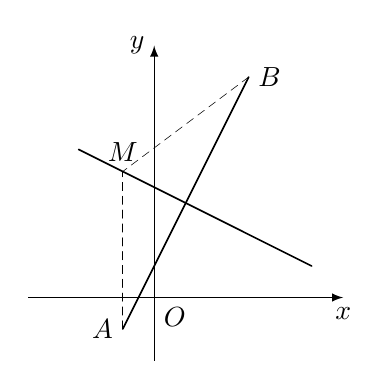
\begin{tikzpicture}[>=latex,scale=0.4]
  % \useasboundingbox(0,-0.2)rectangle(3,0.5);
  \draw[thin,->](-4,0)--(6,0)node[below]{$x$};
  \draw[thin,->](0,-2)--(0,8)node[left]{$y$};
  \tkzDefPoints{-1/-1/A,3/7/B,-1/4/M,0/0/O}
  \tkzDrawSegments[semithick](A,B)
  \tkzDefMidPoint(A,B)\tkzGetPoint{M'}
  \tkzDrawLine[semithick,add =0.7 and 2](M,M')
  \tkzDrawSegments[densely dashed](A,M B,M)
  \tkzLabelPoints[left](A)
  \tkzLabelPoints[above](M)
  \tkzLabelPoints[right](B)
  \tkzLabelPoints[below right](O)
\end{tikzpicture}
\end{document}